\documentclass[10pt,a4paper]{article}

\usepackage[utf8]{inputenc}
\usepackage[margin=1.2in]{geometry}
\usepackage{amsmath}
\usepackage{amsfonts}
\usepackage{graphicx}
\usepackage{hyperref}
\usepackage[nottoc, notlof, notlot]{tocbibind}
\hypersetup{colorlinks=true,citecolor=black,filecolor=black,linkcolor=black,urlcolor=black}
\setlength{\parindent}{0.6cm} 
\setlength{\parskip}{0.10cm}
\usepackage[automark]{scrpage2}
\usepackage{color, colortbl}
\usepackage[table]{xcolor}
\usepackage{hyperref}
\usepackage{listings}
\usepackage{xcolor}


\pagestyle{scrheadings}

\ihead[]{Équipe Navigation}
\ohead[]{Manuel développement}



\begin{document}
\pagestyle {plain}

\begin{titlepage}


\newcommand{\HRule}{\rule{\linewidth}{0.5mm}} 

\center

\textsc{\Large Université Paul Sabatier}\\[1cm] 

\includegraphics[scale=0.3]{figures/UPS.jpg}\\[0.6cm] 


\textsc{Master Intelligence Artificielle et \\ 
Reconnaissance des Formes \\ Master Robotique : Décision et Commande}\\[3cm] 

\HRule \\[0.4cm]
{ \huge \bfseries Manuel développeur}\\[0.4cm] 
\LARGE Navigation Autonome de Robot Mobile

\HRule \\[1.5cm]
 

\begin{minipage}{0.4\textwidth}
\begin{flushleft} \large
\emph{Auteurs:}\\
\href{mailto:thibaut.aghnatios@laposte.net}{Thibaut \textsc{Aghnatios} }  \\
\href{mailto:bouchetmarinee@gmail.com}{Marine \textsc{Bouchet} } \\
\href{mailto:bruno.dato.meneses@gmail.com}{Bruno \textsc{Dato} } \\
\href{mailto:klempka.tristan@gmail.com}{Tristan \textsc{Klempka} } \\
\href{mailto:lagoute.31@gmail.com}{Thibault \textsc{Lagoute} }  
\end{flushleft}
\end{minipage}
~
\begin{minipage}{0.4\textwidth}
\begin{flushright} \large
\emph{Tuteurs:} \\
\href{mailto:lerasle@laas.fr}{Frédéric \textsc{Lerasle}}\\
\href{mailto:michael.lauer@laas.fr}{Michaël \textsc{Lauer}} \\
\href{mailto:taix@laas.f}{Michel \textsc{Taix}}
\end{flushright}
\end{minipage}\\[5cm]

\large 13 mars 2017
 

\end{titlepage}

\newpage


\subsection*{Suivi du document}

\begin{center}
    \begin{tabular}{| l | l | l | l | l |}
    \hline
     \rowcolor{gray} Nom du document & Version Majeure & Version Mineure & Date de création & Dernière version \\ \hline
    Manuel développeur & A & 7 & 13/03/2017 & 4/04/2017 \\ \hline
    \end{tabular}
\end{center}


\subsection*{Auteurs du document}

\begin{center}
    \begin{tabular}{| l | l | l | l |}
    \hline
    \rowcolor{gray} Rédaction & Intégration & Relecture & Validation Interne \\ \hline
    Équipe & Équipe & Bruno Dato & Marine Bouchet \\ 
     &  & Tristan Klempka & \\ \hline

    \end{tabular}
\end{center}

\subsection*{Validation du document}

\begin{center}
    \begin{tabular}{| l | l | l | l |}
    \hline
     \rowcolor{gray} Validation & Nom & Date & Visa \\ \hline
    & & & \\
     \hline
    \end{tabular}
\end{center}

\subsection*{Liste de diffusion}

Le manuel de développement est diffusé à l'ensemble des clients et des intervenants externes aux projets.

\subsection*{Historiques de révision}

\begin{center}
    \begin{tabular}{| l | l | l | l |}
    \hline
     \rowcolor{gray} Version & Modification apportée & Auteur & Date \\ \hline
    A.0 & Création du document & Bruno Dato & 13/03/2017\\ \hline
    A.1 & Sections \ref{sec:introduction} et \ref{sec:navigation_avec_amers_2D_dans_un_environnement_connu} & Marine Bouchet & 27/03/2017\\ \hline
    A.2 & Section \ref{sec:navigation_avec_amers_2D_dans_un_environnement_connu} & Tristan Klempka & 28/03/2017\\ \hline
    A.3 & Section \ref{sec:visibilite} & Thibaut Aghnatios & 30/03/2017\\ \hline
    A.4 & Sections \ref{sec:commande} et \ref{sec:superviseur} & Bruno Dato & 30/03/2017\\ \hline
    A.5 & Section \ref{sec:superviseur} & Bruno Dato & 31/03/2017\\ \hline
    A.6 & Section \ref{sec:introduction} & Bruno Dato & 1/04/2017\\ \hline
    A.7 & Relecture & Bruno Dato & 4/04/2017\\ \hline
     
    \end{tabular}
\end{center}

\newpage
\tableofcontents
\newpage

\section{Introduction}
\label{sec:introduction}

Ce manuel donne les informations nécessaires à l'utilisation et à l'évolution du projet "Navigation autonome d'un robot mobile" du Master 2 IARF et RODECO. Celui-ci permet, à ce jour, d'effectuer une navigation autonome d'un Turtlebot dans un environnement connu, contenant des amers dont leur position et leur orientation sont connus. Ces indices visuels, visualisés par la kinect, capteur RGB-D, permettent de supprimer les erreurs systématiques de la localisation des capteurs proprioceptifs embarqués -- de l'odométrie. 

La navigation s'effectue entre une position initiale, connue ou dans la zone de visibilité d'un amer, et une position finale : 

\begin{center}
\begin{tabular}{c|c|c}
Scénario & A & B \\ \hline
Départ & Position initiale absolue & Position initiale inconnue mais dans une \\ 
  &  & zone de visibilité d'un marqueur \\  \hline
Arrivée & Position finale & Position finale 
\end{tabular}\\
\end{center}


\begin{tabular}{cl}
B & Si pas de position en entrée  \\
  & Le robot effectue une recherche de marqueur dans son champs visuel \\
  & Tant que pas de marqueur en vue \\
  & Le robot tourne sur lui même \\
  & Il effectue une autre recherche de marqueur dans son champs visuel \\
& \\
A & Tant que le but est plus loin que le prochain marqueur dans sa direction \\
  & Le robot se déplace jusqu'à la zone de visibilité du marqueur le plus proche dans la direction du but  \\
  & Le robot effectue une recherche de marqueur dans son champs visuel \\
  & Tant que pas de marqueur en vue  \\
  & Le robot tourne de sur lui même  \\
  & Il effectue un autre recherche de marqueur dans son champs visuel \\
  & Le robot se déplace jusqu'au but  \\
\end{tabular}

Étant donné que la connaissance sur la visibilité d'un marqueur n'es pas encore opérationnelle, on considérera que le robot se trouve toujours dans une zone visibilité. On placera alors le robot dans une zone de visibilité à chaque début de navigation en veillant aussi à donner une position initiale correcte.

\section{Navigation avec amers 2D dans un environnement connu}
\label{sec:navigation_avec_amers_2D_dans_un_environnement_connu}

La tâche de navigation autonome se découpe en six briques : 
\begin{description}
\item [Détection] qui permet de repérer les amers dans le champs de vision quand ils se présentent 
\item [Localisation] qui permet de savoir où se trouve le robot, en utilisant soit les données d'odométrie interne, soit les données d'observation
\item [Trajectoire] qui permet de générer le chemin à suivre pour aller d'un point A à un point B
\item [Commande] qui permet d'assurer le suivi de trajectoire ou d'effectuer des commandes simples en boucle ouverte
\item [Visibilité] qui permet de générer une carte contenant les positions des amers et leurs orientations ; et de renvoyer à partir de cette carte le nombre d'amers visibles 
\item [Supervision] qui gère le bon déroulement de la tâche, le déplacement du point de départ au point d'arrivée 
\end{description}



\subsection{Solution mise en place}
\label{sec:solution_mise_en_place}

L'architecture globale de notre produit est décrite par le schéma suivant :

\begin{figure}[h]
\center
% 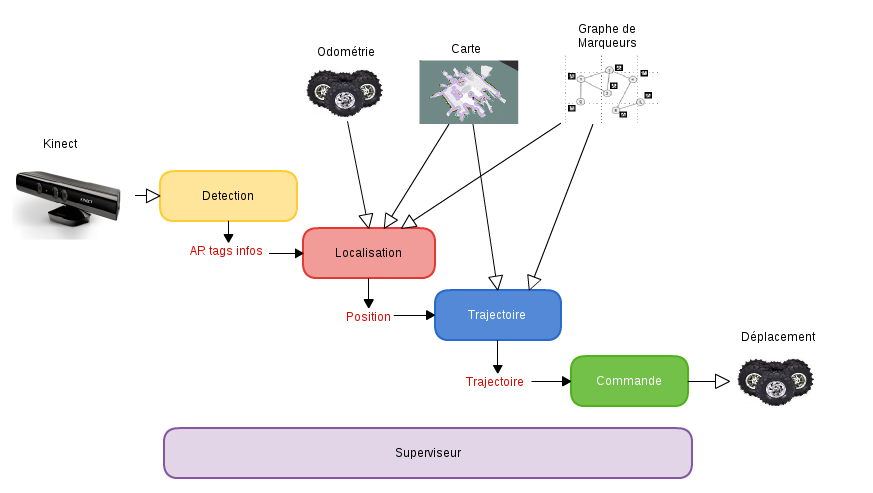
\includegraphics[scale=0.6]{figures/archi.png} 
\caption{Architecture ROS}	
\end{figure}




\subsection{Détection}
\label{sec:detection}

\subsubsection{Fonctionnement}

Afin de détecter les amers dans la scène, nous utilisons à la brique ROS : $ar\_track\_alvar$ qui utilise la librairie open source Alvar pour la détection de marqueurs AR.
Cette brique utilise le nuage de points 3D associé à la couleur pour identifier un marqueur. L'information de profondeur permet à l'algorithme de mieux repérer les plans des marqueurs dans la scène. Elle retourne l'identifiant, la position et l'orientation du marqueur dans le repère de la $/camera\_rgb\_optical\_frame$. La librairie fournie 55 marqueurs AR et la possibilité d'étendre cette liste facilement. Dans notre cas, nous utilisons uniquement le nœud qui permet de lire les marqueurs un par un (individual tags). En effet il existe un autre nœud qui permet d'estimer une position en observant un ensemble de marqueurs (multi-tag bundles).

\subsubsection{Mise en place physique} 
Lors de notre projet nous avons utilisé des marqueurs de taille $16 \times 16$ cm. On place leur milieu à 31 cm du sol afin que l'axe caméra-marqueur soit le plus parallèle au sol possible.

\subsubsection{Utilisation}

 Le nœud de détection est lancé indépendamment des autres nœuds du système. Il s'initialise dans $localisation.launch$ avec les paramètres suivant : 
\begin{itemize}
\item $marker\_size$ : largeur (cm) des marqueurs AR utilisés
\item $cam\_image\_topic$ : topic ROS du flux d'images de la caméra
\item $cam\_info\_topic$ : topic ROS des informations propres à la caméra -- c'est ici que les données de calibrage sont récupérées
\item $output\_frame$ : repère dans lequel sera exprimé le résultat de la détection -- $/camera\_rgb\_optical\_frame$ dans notre cas
\end{itemize}

\subsubsection{Sorties}

Le nœud publie les informations de détection dans des messages de types $ar\_track\_alvar\_msgs::AlvarMarkers$ sur le topic $/ar\_marker\_pose$. Il publie aussi la TF associée au marqueur vu dans le repère de la caméra.
	
\subsubsection{Performances et évolutions}

L'orientation du marqueur trouvé par $ar\_track\_alvar$ doit être : $\vec{z}$ la normale et $\vec{x}$ vers le haut. Il arrive, pour des problèmes inconnus (possiblement le réseau ou des bruits de mesure) que ce repère ne soit pas correctement capturé, avec par exemple, $\vec{y}$ vers le haut. Le robot, à la fin de la localisation se retrouve alors couché. Il faudrait alors comprendre d'où vient le problème ou sinon, ne pas prendre en compte ces orientations aberrantes. 
	
La détection des marqueurs de $16 \times 16$ cm s'effectue jusqu'à 2 m 25 avec une précision de 2 cm et jusqu'à 45 degrés d'angle à 5 degrés près. Il serait intéressant, à l'avenir, d'approfondir les résultats obtenus avec d'autres tailles si l'erreur est trop aléatoire, ou alors, intégrer un filtre de Kalman pour fusionner les données odométriques et les observations.

\begin{figure}
\center

\includegraphics[scale=0.6]{figures/artags.png} 
\caption{Exemple de marqueurs AR. Les valeurs 3, 4 et 5 sont codés avec ces marqueurs.}	
\end{figure}


\subsection{Localisation}
\label{sec:localision}

\subsubsection{Utilisation}
Le nœud de localisation est lancé gr\^ace à un ficher ROS de launch. Cependant, contrairement au nœud de détection, ce nœud ne se lance pas indépendamment des autres. Il est lancé avec l'ensemble du système de navigation avec la commande suivante : \textit{roslaunch turtlebot$\_$proj$\_$nav navigation.launch}

Ce fichier configure et lance le système de navigation qui comprend le nœud de localisation. On trouve dans ce fichier des paramètres propre à la localisation pouvant être configurés.

\begin{itemize}
\item $map\_file$ : Chemin de la carte utilisée pour la navigation. Notre système utilise le nœud ROS $map\_server$ pour le chargement de la carte.
\item $marker\_tf\_publisher\_X$ : L'utilisateur renseigne ici, pour chaque marqueur, la transformée qui sera publiée pour le repérer sur la carte. L'orientation est renseignée avec un quaternion. 
\end{itemize}

\subsubsection{Rappels}
Avant toute chose, il est important de rappeler que quelque soit la situation :
\begin{itemize}
\item $/map \rightarrow /odom \rightarrow /base\_link $ (\url{cf. http://www.ros.org/reps/rep-0105.html})
\item Le repère $/map$ doit être correctement placé en position et en orientation puisque toute les transformations vont se faire à partir de celui-ci.
\item /odom est le repère relatif de l'odométrie, assimilé certain, du robot et est placé au départ sur /map. Il est en quelque sorte le point de départ d'un déplacement. Étant donné que ce repère dérive au cours du déplacement du robot, il peut être erroné. La localisation via un amer connu permet de placer le repère /odom au bon endroit, et de réinitialiser l'odométrie, ce qui place /base\_link au même endroit. C'est une localisation absolue.
\item chaque frame peut avoir plusieurs fils mais qu'un seul parent
\item la transformée entre deux frames est décrite par deux attributs : 
  \begin{itemize}
  \item $m\_origin$ : Vector3 de translation 
  \item $m\_basis$ : Matrix3x3 de rotation
  \end{itemize}
\end{itemize}

\subsubsection{\textit{localisation\_node.cpp}}
Ce nœud permet d'envoyer la nouvelle localisation du robot s'il détecte un marqueur. 

\subsubsection{Traitement}
\noindent La recherche se déclenche uniquement et une seule fois quand la commande de haut niveau publie un $<$std\_msgs::Empty$>$ sur le topic $/nav/HLC/askForMarker$. 

\noindent Dans le cas ou un marqueur est visible, voici le processus : 
\begin{itemize}
\item On sait à priori : /map $\rightarrow$ /odom $\rightarrow$ /baselink $\rightarrow$ /camera\_rgb\_frame $\rightarrow$ /camera\_rgb\_optical\_frame 
\item À l'arrivée d'un marqueur, on a : /camera\_rgb\_optical\_frame $\rightarrow$ /ar\_marker\_ID 
\item On remonte l'information : /baselink $\rightarrow$ /camera\_rgb\_frame $\rightarrow$ /camera\_rgb\_optical\_frame $\rightarrow$ /ar\_marker\_ID
\item On sait donc : /ar\_marker\_0 $\rightarrow$ /baselink, qui est égal à /marker\_0 $\rightarrow$ /baselink 
\item Sachant /map $\rightarrow$ /marker\_0, on sait /map $\rightarrow$ /baselink = /map  $\rightarrow$ /odom 
\end{itemize}

Cette transformation est envoyée sur $/new\_odom$ que l'on publie avec le publisher $odom\_pub$. On publie également l'identifiant du marqueur vu sur $/nav/loca/markerSeen$ sous un $<$std\_msgs::Int16$>$. 

\noindent Dans le cas où on ne voit rien on publie : -1 

\subsubsection{Initialisation}
\noindent Différents champs peuvent être paramétrés : 
\begin{itemize}
\item $DEBUG$ : Active ou non les sorties de debug. Si cette option est activée, les transformations intermédiaires sont publiées.
\item $TIMEOUT\_AR\_DETEC$ : Temps d'attente maximum pour la réception d'un marqueur. Ce paramètre est utile lors de l'utilisation en réseau. La latence provoque des retards dans la publication des transformées. Il est donc nécessaire de donner une marge de temps au système. Lors de l'utilisation en mode local cette valeur peut \^etre faible.
\item $NB\_MARKER$ : Nombre de marqueurs total dans la scène.
\end{itemize}

Une fois le lancement du nœud effectué, l'utilisateur peut observer son comportement avec des sorties console :
\begin{itemize}
\item $GLOBAL\_SEARCH$ : La recherche de marqueur a été demandée.
\item $ MARKER DETECTED: ID\_MARKER\_DETECTED$ : Identifiant du marqueur détecté.
\item $LOOKING FOR TF: tf$ : Nom de la transformée attendue.
\end{itemize}

\subsubsection{Améliorations}
Il serait préférable de récupérer les TFs /baselink $\rightarrow$ /camera\_rgb\_frame et /camera\_rgb\_frame $\rightarrow$ /camera\_rgb\_optical\_frame en dynamique plutôt qu'en statique, de même pour le nombre de marqueurs dans la scène.

\begin{figure}
\center\noindent
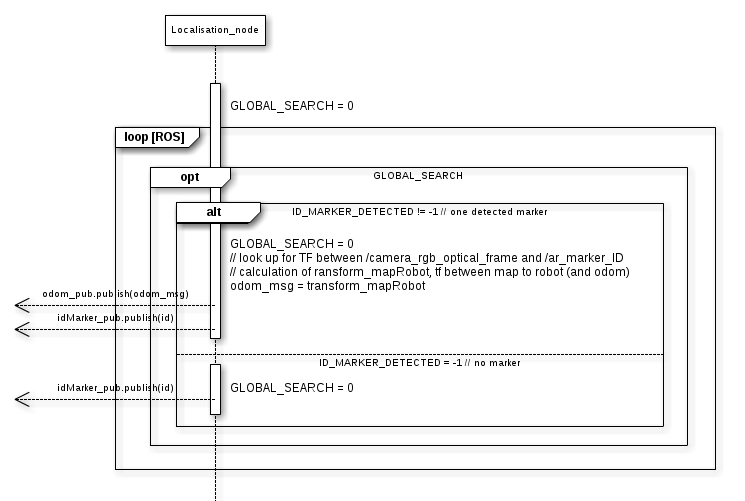
\includegraphics[scale=0.6]{figures/locaprocess.png} 
\caption{Traitement général lors de la localisation}	
\end{figure}

\begin{figure}
 \begin{minipage}[b]{.48\linewidth}
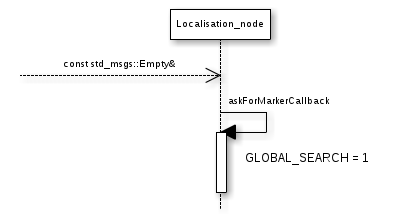
\includegraphics[scale=0.5]{figures/locacbask.png} 
  \caption{Callback de la demande de localision}
 \end{minipage} \hfill
 \begin{minipage}[b]{.46\linewidth}
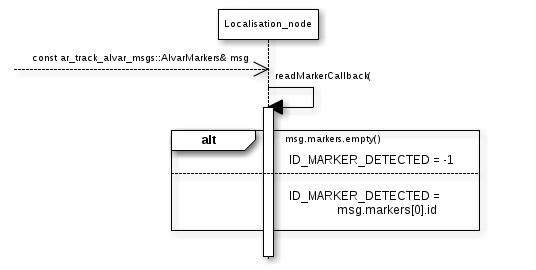
\includegraphics[scale=0.5]{figures/locacb2read.png} 
  \caption{Callback du résulat de la détection}
 \end{minipage}
\end{figure}
\subsubsection{\textit{localisation\_broadcaster\_node.cpp}}

Ce nœud permet de tout le temps diffuser la transformée entre $/map$ et $/odom$. Il souscrit à la $<geometry\_msgs::Transform>$ /new\_odom, qui contient la "nouvelle" position certaine du robot. Dès que celle-ci est publiée, $/odom$ actualise sa position et on réinitialise le $nav\_msgs/Odometry$ : il devient notre nouveau référentiel.

\begin{figure}
\center
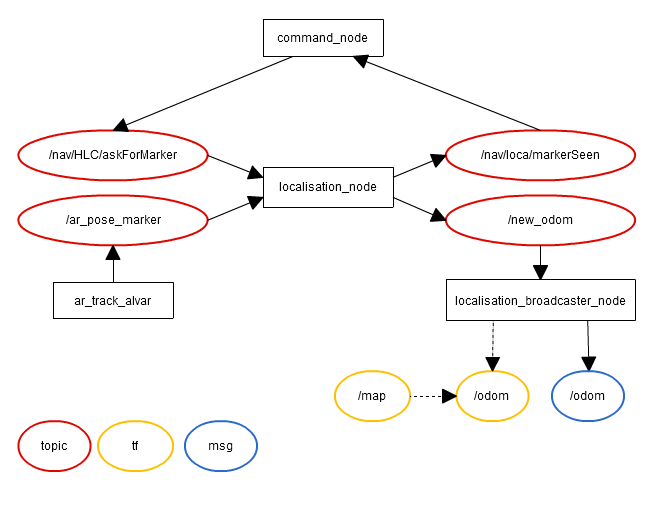
\includegraphics[scale=0.6]{figures/rqt_loca.png} 
\caption{texte de la légende}	
\end{figure}




\subsection{Commande}
\label{sec:commande}
\subsubsection{Utilisation}

Pour la version actuelle du projet, la plupart de la commande est effectué par une brique ROS. La brique $move\_base$ réalise la commande afin de suivre la trajectoire générée par la brique trajectoire. Cette brique est lancé dans un fichier ROS de launch.\\
\textit{roslaunch turtlebot$\_$proj$\_$nav navigation.launch}\\
La commande peut être configurée à l'aide du fichier XML : \textit{move\_base.launch.xml}. Ce fichier XML référence un ensemble de fichiers XML qui configure la commande. Une description exhaustive des paramètres de cette brique peut être trouvée à cette adresse :\\
\textit{http://wiki.ros.org/move\_base}\\
Lors de la recherche d'un marqueur, nous reprenons la main et c'est la nœud $commande\_node$ qui prend le relais. Celle-ci est également lancée dans $navigation.launch$.

\subsubsection{Fonctionnement}

Au début du projet une ébauche de commande a été réalisée. Celle-ci est simple, elle permet un déplacement en ligne droite et une rotation sur place. Cette commande est en boucle ouverte. Il peut \^etre intéressant de continuer ce travail afin de prendre en compte une correction odométrique notamment lors d'un évitement d'obstacle lorsque le système reprend la main sur la commande de suivi de trajectoire faite par la brique $move\_base$.\\
Cette ébauche ce trouve dans le fichier $commande\_node.cpp$ \\
Cette node est lancée dans le fichier ROS de launch $navigation.launch$.\\

La commande simple était à la base prévu pour la chercher d'une balle de couleur, une fois sa position repérée. Le but était de faire tourner le robot pour s'orienter face à la balle et ensuite d'avancer vers la balle. Nous avons alors repris cette commande pour exécuter les comportement de rechercher de marqueurs. On utilise alors seulement les rotations.

\begin{figure}[!h]
\centering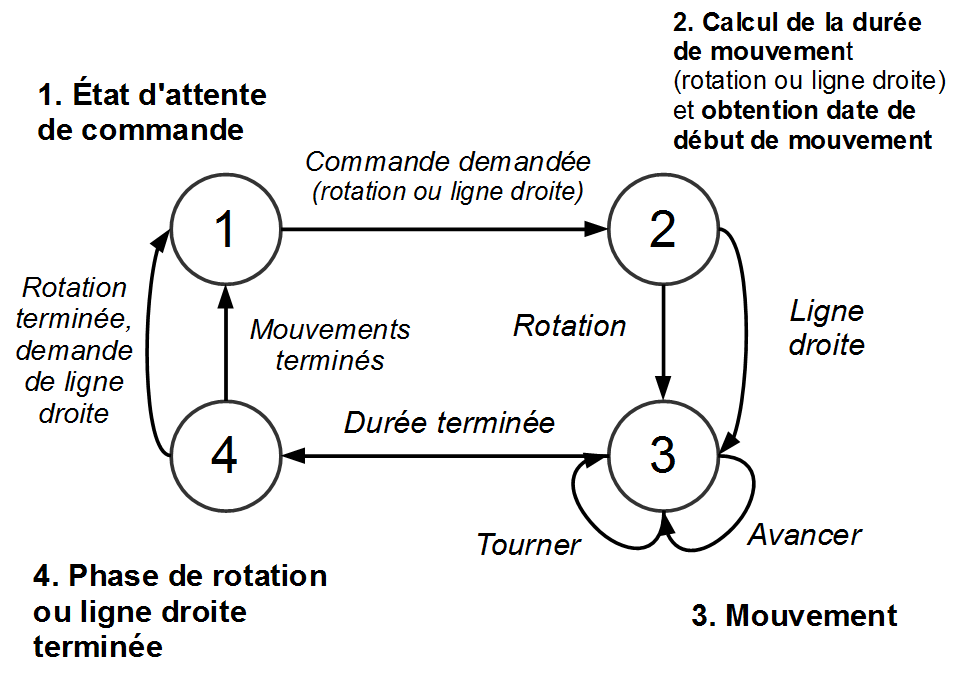
\includegraphics[scale=0.4]{figures/commande_MEF.png}
\caption{Schéma de la machine à états de la commande utilisée pour la recherche d'une balle et pour la recherche d'un amer}
\label{commande_MEF}
\end{figure}

\subsection{Visibilité}
\label{sec:visibilite}

Le but de cette section est de créer et d'utiliser une carte de visibilité, une carte contenant l'ensemble des positions où le robot voit au moins un des amers, afin de retourner le nombre d'amers visibles pour une position donnée. L’intérêt de cette carte est de pouvoir suivre notre navigation d'amers en amers et de savoir si l'on se trouve dans un champ de visibilité pour lancer la détection et la localisation avec notre superviseur.

Nous expliquons ici comment la carte de visibilité est générée, à l'aide de $visib\_pgmwriter\_node.cpp$, et le mécanisme de la node $visib\_pgmreader\_node.cpp$, retournant le nombre d'amers visibles.

\subsubsection{Génération de la carte de visibilité}
Tout d'abord pour générer la carte de visibilité, il faut au préalablement avoir une carte de l'environnement. Cette carte est créée virtuellement ou en utilisant la cartographie disponible sur le Turtlebot, utilisé dans le $map\_server$.

\begin{figure}[!h]
\center
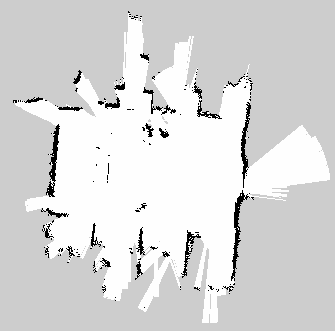
\includegraphics[scale=0.6]{figures/aip_map.png} 
\caption{Cartographie de l'environnement avec le Turtlebot}	
\end{figure}

Le node $visib\_pgmwriter\_node.cpp$ ne doit pas être modifié, toutes les configurations se font directement dans le fichier $visib\_init.cpp$. En effet, le node lance la fonction $Ecriture\_carte\_visib()$ qui crée dans un fichier au format PGM (Plain PGM : $http://netpbm.sourceforge.net/doc/pgm.html\#plainpgm$) l'ensemble des amers définit dans le $graph.xml$ se trouvant dans le dossier $/rsc$. Donc pour une taille de carte donnée et pour les configurations effectuées correctement dans $visib\_init.cpp$  expliquées par la suite, il suffit de modifier la position et l'orientation de nos amers dans le $graph.xml$ (voir partie 2.6.2) pour que la nouvelle carte de visibilité soit générée automatiquement en lançant à nouveau notre node $visib\_pgmwriter\_node.cpp$.\\

\begin{figure}[!h]
\center
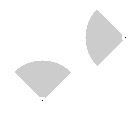
\includegraphics{figures/visib.png} 
\caption{Exemple d'une carte de visibilité}	
\end{figure}

Une fois notre carte générée, il faut pouvoir la visualiser sur Rviz et la superposée avec la carte de notre environnement pour qu'elle soit plus parlante. En lançant le $navigation.launch$ notre carte de visibilité est publiée sur le topic $\/markers\_visibility\_map$. Il suffit de l'ajouter directement sur Rviz en ajoutant celle-ci et en se plaçant sur le topic en question. Le résultat obtenu sur Rviz est le suivant :

\begin{figure}[!h]
\center
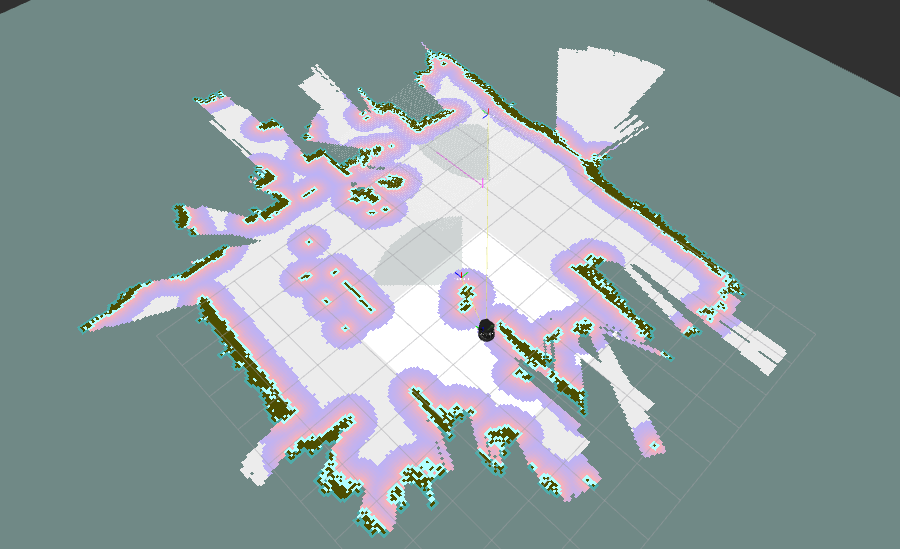
\includegraphics[scale=0.4]{figures/visib_rviz.png} 
\caption{Superposition de nos cartes sur Rviz}	
\end{figure}

Au niveau de la configuration de $visib\_init.cpp$ dans la fonction $Ecriture\_carte\_visib()$, il faut modifier $int largeur=512;	 int hauteur=640;$ pour que la carte aie toujours les mêmes dimensions que la carte de notre environnement. $int nbr_amers=2;$ pour prendre en compte le nombre d'amers contenus dans $graph.xml$. Ensuite dans la boucle $for$ faisant la conversion de la position de mètre en pixels :

$\\
for(a=0;a<nbr\_amers;a++)\\
	\{ \\
. \hspace{35pt}    x[a]=(x1[a]+12.2)/0.05;\\
. \hspace{35pt}    y[a]=-(y1[a]+13.8-32)/0.05;\\
. \hspace{35pt}    alphamax[a]=pi/4;\\
	\}\\
	$


Avant tout, il faut savoir qu'on a 3 repères différents.\\ 
- On a le repère du robot que l'on nomme R et possède la position en x et y du robot donc R (X,Y).\\
- Le repère de la carte de l'environnement note R' qui a pour origine (-12.2 ; -13.8) (dans notre cas pour une carte 512 x 640) donc R' (X+12.2, Y+13.8).\\ 
- Ensuite on a le repère de notre carte de visibilité noté Rp qui est positionné en haut a gauche de la carte (vecteur u dans le même sens que x et vecteur v opposé au vecteur y) c'est pourquoi on peut écrire Rp (X+12.2, -(Y+13.8-32)).\\

Explicitons maintenant les différentes valeurs utilisées : 0.05 correspond à la résolution qui se trouve dans le fichier de configuration .yaml dans $/map$. Ici 12.2 et 13.8 correspond à l'origine de la carte pour que la superposition des cartes soit correctes. En effet, si on laisse 0.0 et 0.0, la carte se générera à la base du robot sur Rviz donc on aura un décalage lors de la superposition. C'est pourquoi dans le fichier $visib.yaml$, il faut aussi le configurer de cette manière pour notre cas :\\
$resolution: 0.050000\\
origin: [-12.200000, -13.800000, 0.000000]\\
$

Donc, cela permet de passer du repère du robot au repère de la carte pour placer nos marqueurs et créer notre carte de visibilité. Pour le moment les modifications se font manuellement, mais pour améliorer notre programme, il faudrait récupérer nos différentes valeurs (résolution, origine du repère, etc...) directement dans le fichier $.yaml$.\\

Enfin, la valeur 32 correspond à la conversion pixel/mètres de la hauteur de notre fenêtre en faisant :\\ $640*0.05=32$.\\
\\
Ainsi, on peut écrire :

$\\
for(a=0;a<nbr\_amers;a++) ~\\
	\{  ~\\
. \hspace{35pt}    x[a]=(x1[a]+12.2)/0.05; ~\\
. \hspace{35pt}    y[a]=-(y1[a]+13.8-32)/0.05; ~\\
. \hspace{35pt}    alphamax[a]=pi/4; ~\\
	\} ~\\
	$

\subsubsection{Noeud retournant le nombre d'amers visibles}
Maintenant que nous possédons une carte de visibilité, le nombre d'amers visibles de la position du robot est renvoyé à l'aide de la node $visib\_pgmreader\_node.cpp$. Il lit le fichier PGM créé et renvoie la valeur du pixel pour une position (x,y) sur cette carte (on utilise le topic MarkersVisibility). Si le pixel vaut 15 on est dans une zone blanche donc pas de marqueurs visibles. Pour un pixel de valeur 12, cela veut dire qu'on est dans le champ de visibilité d'un amer. Pour 9, 2 amers visibles. Pour 6, 3 amers visibles. Pour 3, 4 amers visibles. Ensuite pour 5 amers visibles, le pixel passe à 0, cependant on ne peut plus distinguer si le pixel est à 0 car 5 amers visibles ou bien car il s'agit du pixel correspondant à l'amer. C'est pourquoi dans notre cas, on suppose qu'au maximum 4 amers sont visibles en même temps. 
Si on souhaite avoir plus d'amers visibles en même temps, il suffit d'augmenter la valeur maximale lors de l’écriture de la carte de visibilité. En effet, lors de la création de l’entête PGM, on définit la valeur maximale de nos pixels (dans notre cas 15).\\

ATTENTION : nous n'avons pas réussi à la rendre fonctionnelle lors de notre intégration. Lors des tests avant intégration, le node suivant renvoyé bien le nombre d'amers visibles, cependant en l'intégrant, notre fonction $pgm\_imread(char *argv)$ ne stocke plus correctement les valeurs des données. Il faut donc la débugger avant qu'elle soit utilisée.

\newpage
\subsection{Superviseur}
\label{sec:superviseur}

\subsubsection{Comportement de la navigation}

Le but du superviseur est de guider le robot pour qu'il atteigne un but de coordonnées $(x,y)$ dans la carte. Afin de gérer le comportement de la navigation à l'aide des amers, pour atteindre ce but précis, nous avons mis en place un nœud ROS de supervision : $hightLevelCommand\_node$. Ce nœud permet d'utiliser des commandes de haut niveau telles que \textit{chercher un amer} ou bien \textit{se déplacer vers un but}.\\

(TODO : but absolu : ça suffit pas "Le but du superviseur est de guider le robot pour qu'il atteigne un but de coordonnées $(x,y)$ dans la carte" ?)

On suppose alors qu'initialement, le robot est dans une position connue et dans une des zones de visibilité car notre système ne permet pas à ce jour de le vérifier. Si sa position est assez proche du but final suivant un seuil que l'on définira par la suite, on commande alors au robot de se déplacer directement vers le but. Si la position initiale est trop éloignée, on se déplace d'amer en amer pour atteindre l'amer qui est le plus proche du but final pour enfin se déplacer vers le but final. Tous les amers et les distances entre ces derniers sont représentés par un graphe, ainsi on utilise l'algorithme de plus court chemin Dijkstra pour déterminer vers quel amer se déplacer. Ce graphe est re-calculé à chaque fois que l'on voit un amer.\\

Le comportement détaillé du superviseur est décrit par une machine à états décrite dans la figure \ref{HLC_MEF}.



\begin{figure}[!h]
\centering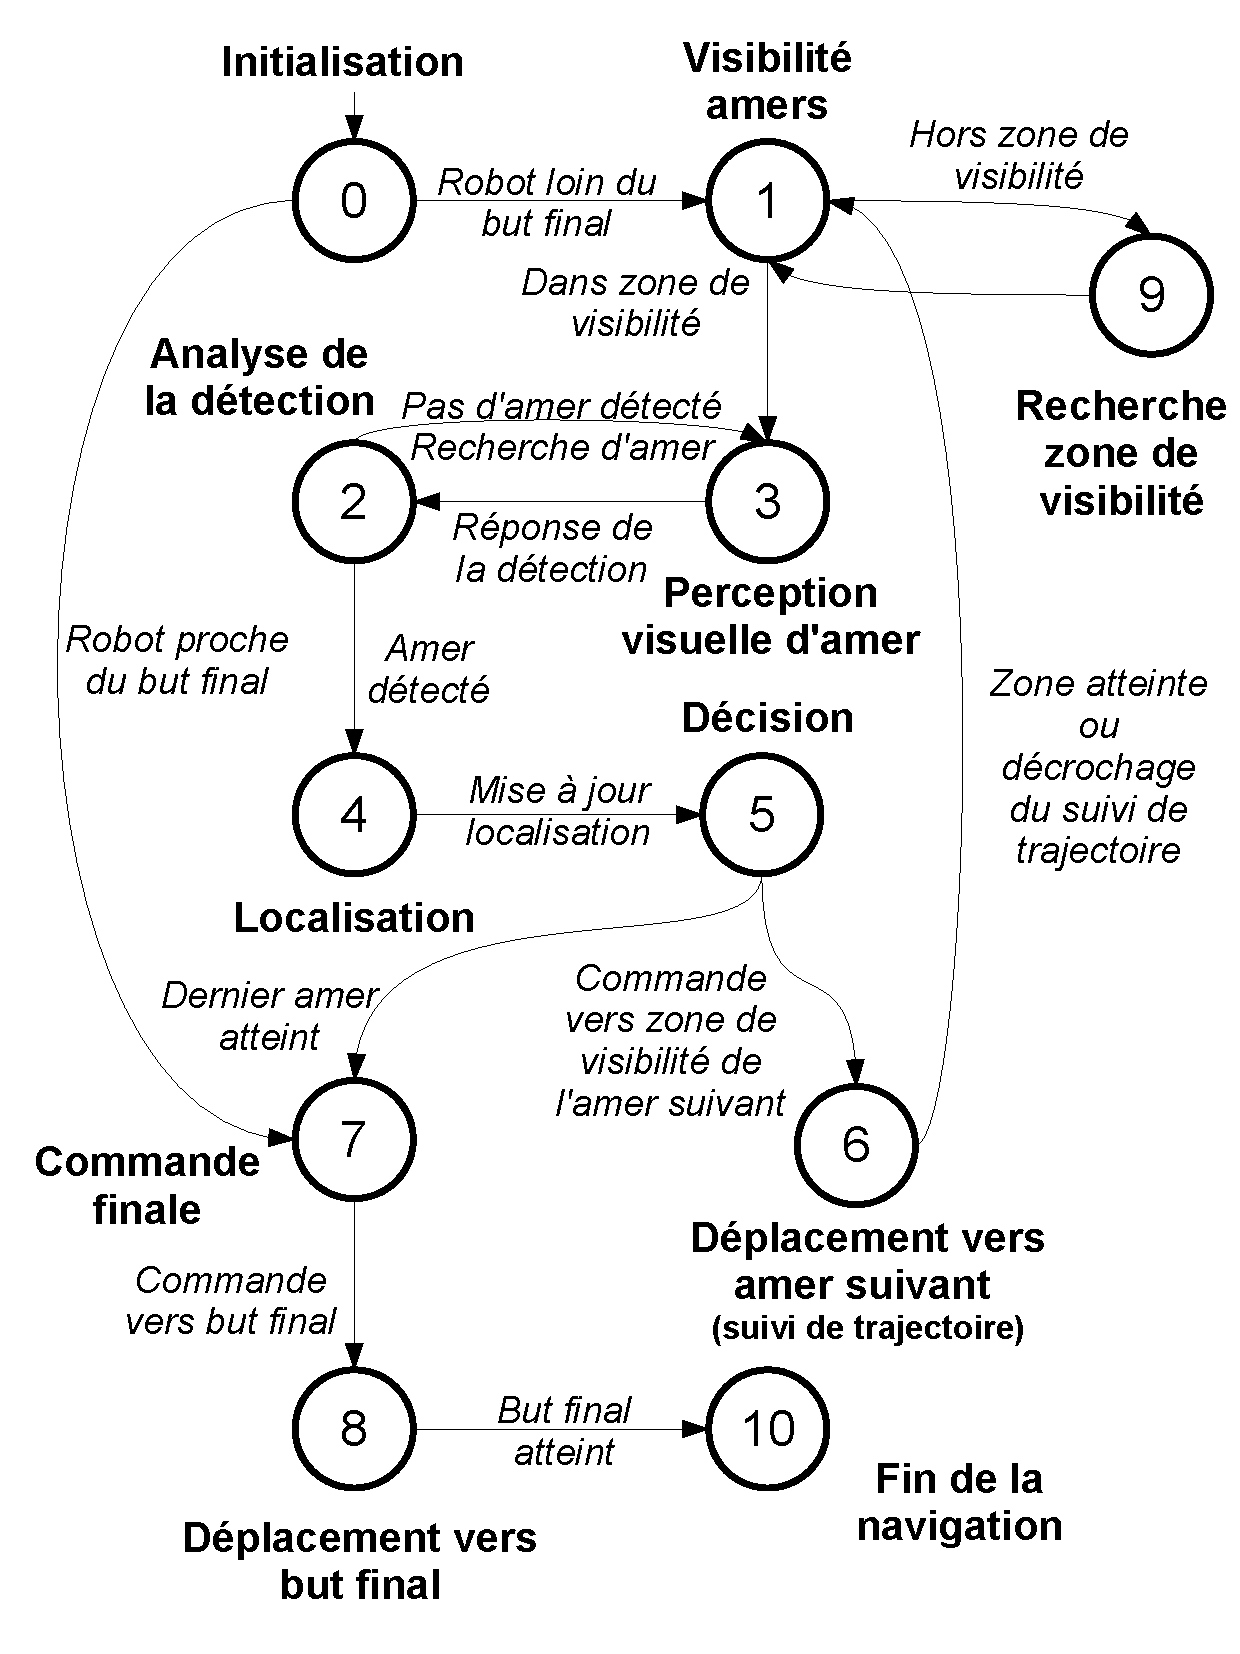
\includegraphics[scale=0.5]{figures/HLC_MEF.pdf}
\caption{Schéma de la machine à états du superviseur de la navigation entre amers}
\label{HLC_MEF}
\end{figure}

Lors de la navigation, quatre signaux sonores permettent de connaître l'état de la navigation. Ils ont lieu lorsqu'un marqueur est détecté, lorsque le robot a atteint un but intermédiaire ou final et lorsque le robot décroche de sont suivi de trajectoire. Si le robot atteint sont but final avec une précision inférieure à celle demandée au lancement du superviseur, un son supplémentaire est joué.\\

La recherche d'une zone de visibilité n'a pas encore été implémentée. Dans le cas où l'on connait la position initiale du robot dans la carte, il faudrait alors lui commander de se déplacer vers la zone de visibilité la plus proche et alors entamer la recherche de marqueur comme dans le scénario habituel. Dans le cas où cette position est inconnue, il faudrait tout d'abord mettre en place une détection d'obstacles pour pouvoir évoluer dans un environnement inconnu jusqu'à trouver un marqueur.

\subsubsection{Graphe des amers}
\label{sec:grapheDesAmers}

Pour choisir vers quel amer (AR marqueur) se déplacer lorsque l'on en a détecté un et que l'on se trouve encore trop loin du but final pour de diriger directement vers celui-ci, on utilise un graphe représentant tous les marqueurs (figure \ref{graphe}) définis dans un fichier de format XML (figure \ref{graphe_xml}). Chaque nœud du graphe possède différentes propriétés : 

\begin{itemize}
\item[•] Id : numéro correspondant au marqueur AR ; 
\item[•] Label : nom du nœud, chaque nœud correspond à un marqueur AR ; 
\item[•] PositionX : coordonnée selon l'axe x de la carte connue de l'environnement ; 
\item[•] PositionY : coordonnée selon l'axe y de la carte connue de l'environnement; 
\item[•] Orientation : angle entre la normale du marqueur AR et l'axe x de la carte (entre 0 et 2$\pi$).
\end{itemize}

Les numéros permettent de se situer dans le graphe lorsque l'on détecte un marqueur et ainsi trouver le marqueur suivant à atteindre pour continuer la navigation. Les coordonnées $(x,y)$ des marqueurs permettent de connaître les positions à atteindre dans la carte. L'orientation permet de commander au robot de se déplacer en face et à une certaine distance du marqueur pour ne pas foncer dans un mur.

\begin{figure}[!h]
\centering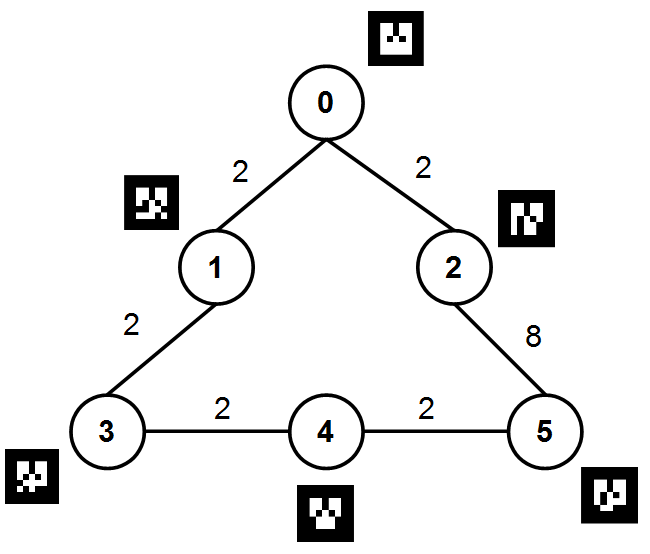
\includegraphics[scale=0.4]{figures/graphe.png}
\caption{Exemple de graphe d'amers (marqueurs AR)}
\label{graphe}
\end{figure}

\begin{figure}[!h]
\centering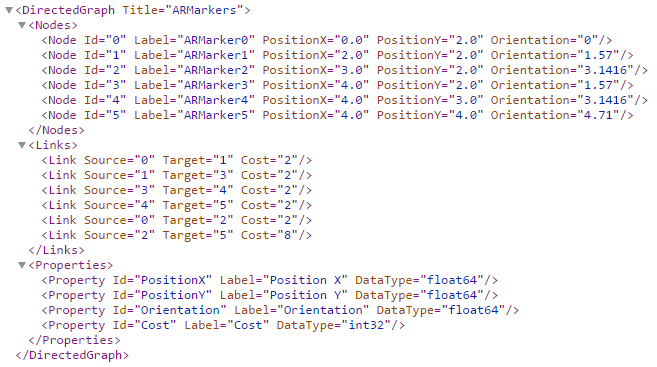
\includegraphics[scale=0.7]{figures/graphe_xml.png}
\caption{Exemple de définition d'un graphe d'amers (marqueurs AR) en format XML}
\label{graphe_xml}
\end{figure}

\newpage
\subsubsection{Commandes de haut niveau}
\label{sec:commandesDeHautNiveau}

Pour mener à bien la navigation, le superviseur utilise la classe $HighLevelCommand$ qui fournit les commandes de haut niveau suivantes :

\begin{itemize}
\item[•] \textbf{init(threshold)} : L'initialisation permet de définir, suivant le seuil (\textbf{threshold}) choisi en paramètre, si le robot est trop éloigné ou non du but final pour se servir des marqueurs durant la navigation. Si le robot est trop proche, la fonction \textbf{init} renvoie $-1$, le superviseur commandera alors au robot de se déplacer directement vers le but final à l'aide de la fonction \textbf{sendFinalGoal()}. Dans le cas contraire, la fonction cherche le marqueur le plus proche du but final, navigue jusqu'à celui-ci, avant d'envoyer la dernière commande vers le but final.
\item[•] \textbf{seekMarker()} : Cette fonction permet de commander le comportement de la recherche d'un amer. Tant que cette méthode est appelée et qu'aucun marqueur n'a été détecté, le robot tourne successivement sur lui-même de $\pi/4$, $-\pi/2$, $3\pi/4$, $-\pi$, $5\pi/4$, $-3\pi/2$ ou $7\pi/4$. Si aucun marqueur n'a été détecté après toutes les rotations, la recherche recommence.
\item[•] \textbf{sendMarkerGoal(distanceToMarker)} : Cette méthode permet de commander au robot de se déplacer en face du marqueur suivant à atteindre pour suivre le plus court chemin vers le but final. La distance à respecter par rapport au marqueur est définie par le paramètre \textbf{distanceToMarker}. 
\item[•] \textbf{sendFinalGoal()} : Cette fonction commande directement le robot vers le but final, choisi à l'instanciation de la classe $HighLevelCommand$.
\item[•] \textbf{askForMarker()} :  Cette méthode permet de lancer une recherche visuelle de marqueur, effectuée par le nœud de localisation.
\item[•] \textbf{finalGoal(threshold)} : Permet de jouer un signal sonore spécial lorsque l'écart entre la position finale du robot et le but fixé est inférieur à un certain seuil, défini à l'aide du paramètre \textbf{threshold}.
\end{itemize}

\newpage
\subsubsection{Structure logicielle}
\label{sec:StructureLogicielle}

Afin de communiquer avec les différents nœuds, le nœud de supervision $hightLevelCommand\_node$ est client d'un service, il publie sur quatre topics et il est abonné à quatre autres topics.


\begin{figure}[!h]
\centering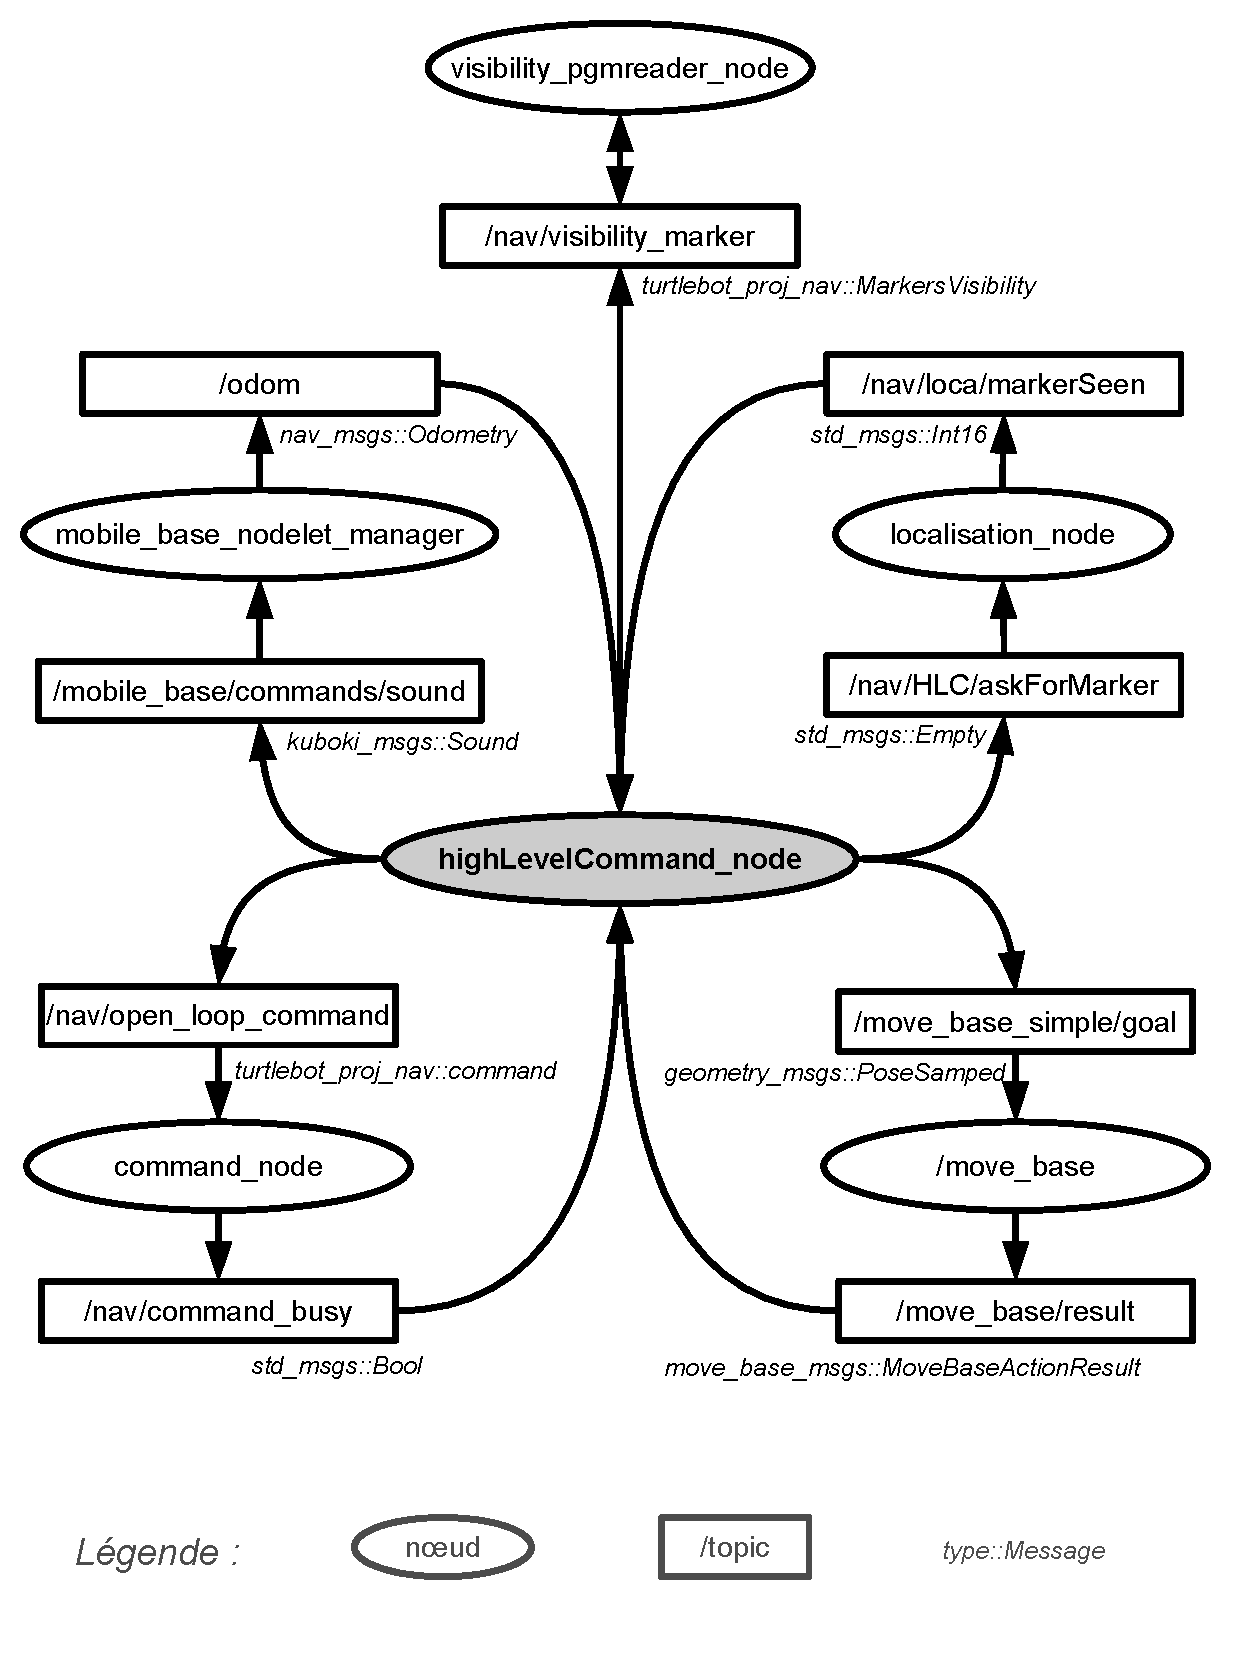
\includegraphics[scale=0.6]{figures/HLC_ROS_struc.pdf}
\caption{Schéma de la structure logicielle du nœud de supervision et de ses interactions }
\label{HLC_ROS_struc}
\end{figure}

\subsubsection{Lancement du superviseur}
\label{sec:LancementDuSuperviseur}

Une fois la configuration minimale et les nœuds de navigation lancés, on lance le superviseur dans un terminal à l'aide de la commande suivante :\\

\textbf{rosrun turtlebot$\_$proj$\_$nav highLevelCommand$\_$node X$\_$GOAL Y$\_$GOAL XY$\_$THRESHOLD XY$\_$PRECISION DISTANCE$\_$TO$\_$MARKERS}\\

\noindent avec les paramètres suivant : 
\begin{itemize}
\item[•] \textbf{X$\_$GOAL} et \textbf{Y$\_$GOAL} : les coordonnées $(x,y)$ du but final à atteindre dans la carte ; 
\item[•] \textbf{XY$\_$THRESHOLD} : le seuil à partir duquel les amers ne sont pas utilisés pour la navigation ; 
\item[•] \textbf{XY$\_$PRECISION} : la contrainte de précision demandée pour que le signal sonore final soit joué ou non ; 
\item[•] \textbf{DISTANCE$\_$TO$\_$MARKERS} : la distance par rapport aux marqueurs que le robot doit respecter lorsqu'il se déplace d'amer en amer.
\end{itemize}


\newpage
\section{Conclusion}
\label{sec:conclusion}

\newpage
\listoffigures
\newpage

\section*{ANNEXE}





\end{document}

